\documentclass[11pt, a4paper]{article}

\usepackage{amsmath}
\usepackage{amsfonts}
\usepackage{graphicx}
\usepackage[export]{adjustbox}
\usepackage{hyperref}
\usepackage{fullpage}
\usepackage{caption}
\usepackage{listings}
\usepackage[dvipsnames]{xcolor}
\usepackage{gensymb}
\hypersetup{
    bookmarks=true,         % show bookmarks bar?
    unicode=false,          % non-Latin characters in Acrobat’s bookmarks
    pdftoolbar=true,        % show Acrobat’s toolbar?
    pdfmenubar=true,        % show Acrobat’s menu?
    pdffitwindow=false,     % window fit to page when opened
    pdfstartview={FitH},    % fits the width of the page to the window
    pdftitle={My title},    % title
    pdfauthor={Author},     % author
    pdfsubject={Subject},   % subject of the document
    pdfcreator={Creator},   % creator of the document
    pdfproducer={Producer}, % producer of the document
    pdfkeywords={keyword1, key2, key3}, % list of keywords
    pdfnewwindow=true,      % links in new PDF window
    colorlinks=true,       % false: boxed links; true: colored links
    linkcolor=Blue,          % color of internal links (change box color with linkbordercolor)
    citecolor=green,        % color of links to bibliography
    filecolor=magenta,      % color of file links
    urlcolor=red           % color of external links
}

\title{MAAS - Assignment-02\\
Proposed Architecture for \\Flying Saucers Bakery Project}
\author{Sushant Vijay Chavan\\Ahmed Faisal Abdelrahman\\Abanoub Abdelmalek}
\date{\today}

\begin{document}
\maketitle
\newpage
%\tableofcontents{}
\newpage

\section{The Architecture}
\begin{figure}[h!]
	\centering
	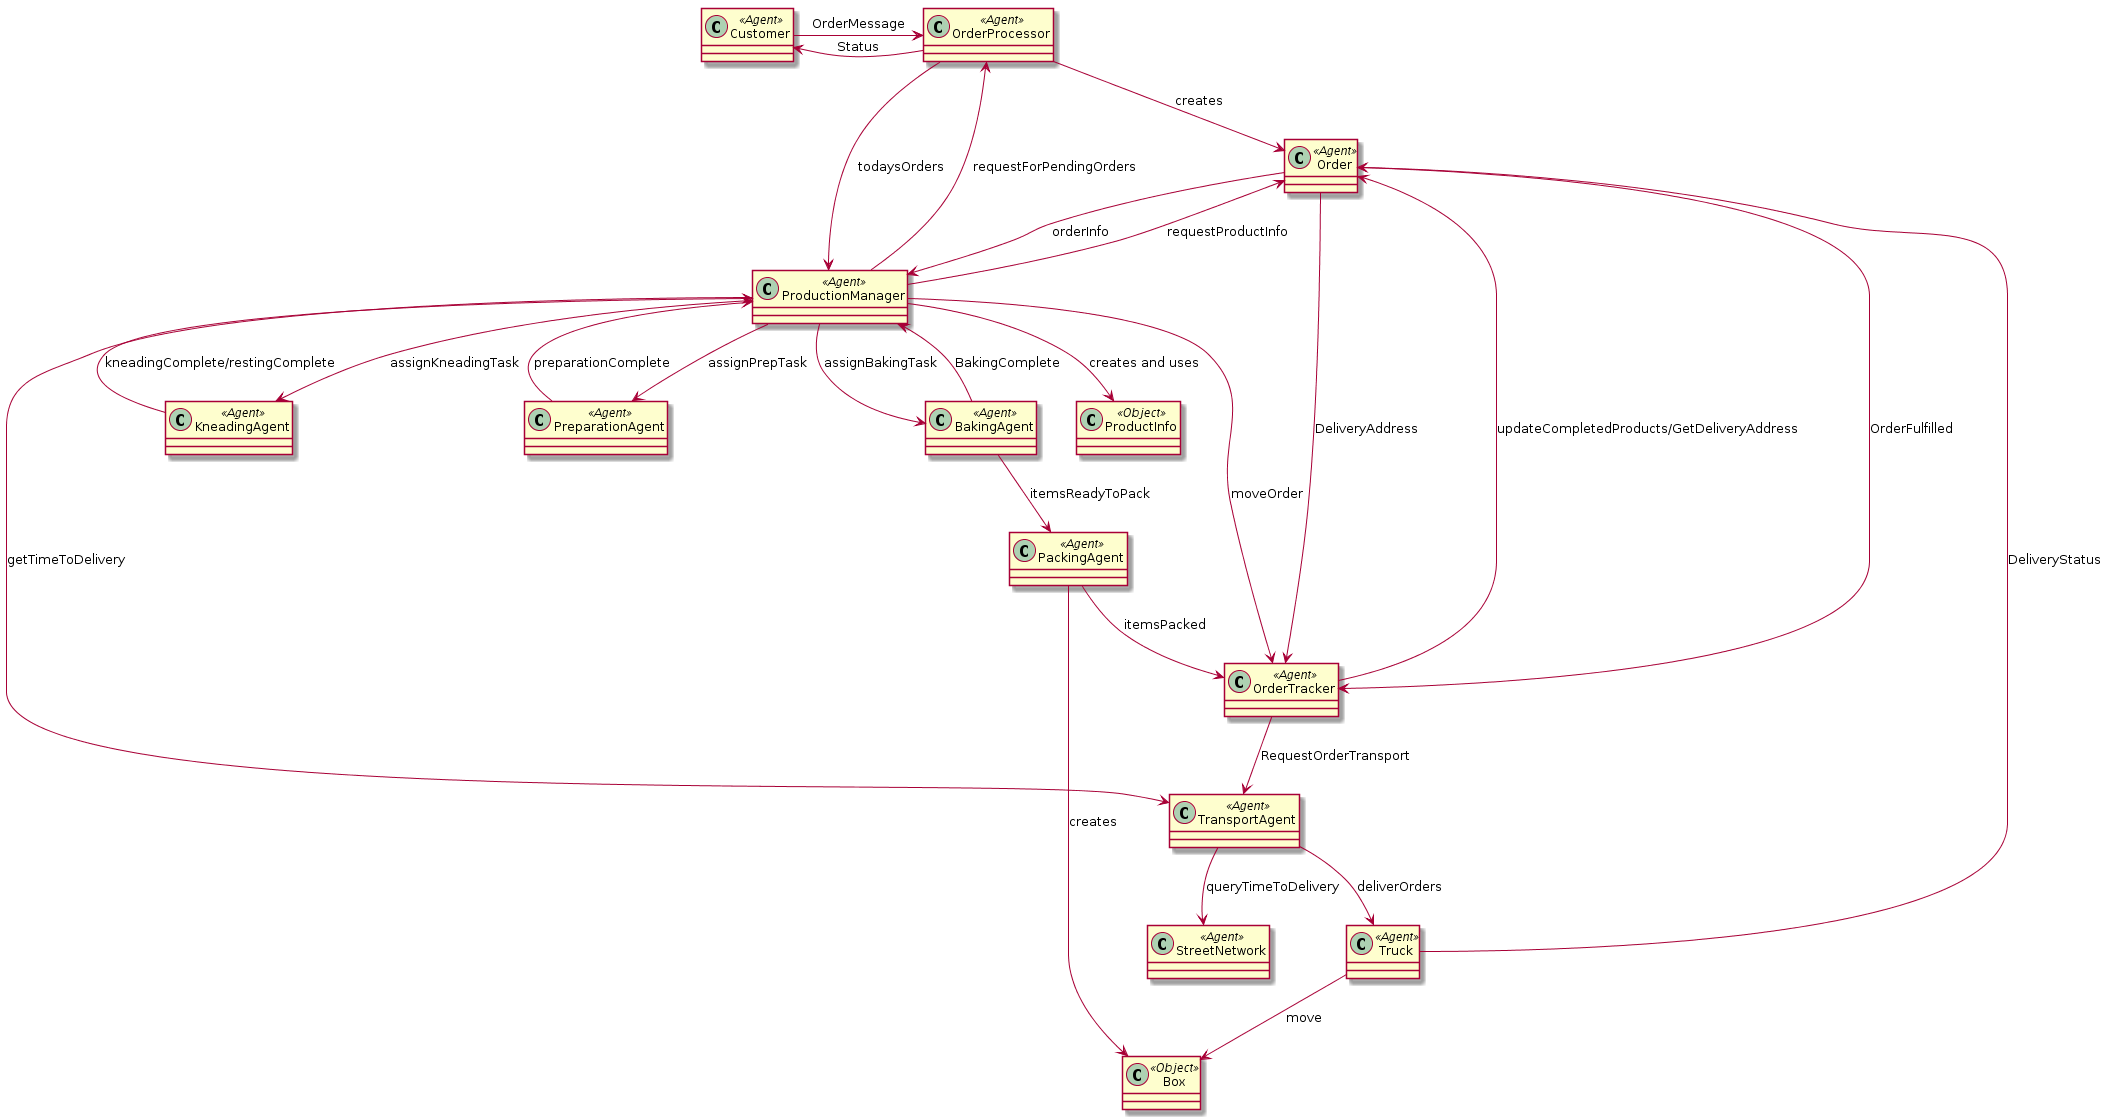
\includegraphics[angle=90, scale=0.27]{../Bakery.png}
	\caption{Architecture diagram}
	\label{Architecture diagram}
\end{figure}
The above figure \ref{Architecture diagram} outlines the overall architecture for the Flying Saucers Bakery project. The tags  above each of the components describe if the component is an object or an agent. The links between the components, represent the messages exchanged between the components. A detailed description of these messages can be looked up in the \textit{Messages.md} file.

\section{Agent Definitions}

The below table  lists out the details of each of the component that are a part of the architecture diagram.
\begin{table}[h!]
\centering
\begin{tabular}{|l|l|l|}
\hline
\textbf{Component} & \textbf{Agent/Object} & \textbf{Static/Dynamic Creation} \\ \hline
Customer           & Agent                 & Dynamic                          \\ \hline
Order              & Agent                 & Dynamic                          \\ \hline
Truck              & Agent                 & Static                           \\ \hline
StreetNetwork      & Agent                 & Static                           \\ \hline
OrderProcessor     & Agent                 & Static                           \\ \hline
ProductionManager  & Agent                 & Static                           \\ \hline
KneadingAgent      & Agent                 & Static                           \\ \hline
PreparationAgent   & Agent                 & Static                           \\ \hline
BakingAgent        & Agent                 & Static                           \\ \hline
OrderTracker       & Agent                 & Static                           \\ \hline
PackingAgent       & Agent                 & Static                           \\ \hline
TransportAgent     & Agent                 & Static                           \\ \hline
ProductInfo        & Object                & Static                                 \\ \hline
Box                & Object                & Dynamic                          \\ \hline
\end{tabular}
\label{Agent Definition}
\caption{Agent Definitions}
\end{table}

\section{Aggregation of order data}

\end{document}\grid
